\documentclass{homework}

\usepackage{graphicx}
\usepackage{minted}
\usepackage{xspace}


\newcommand{\kat}{Kathará\xspace}
\newcommand{\opn}{OPNsense\xspace}
\newcommand{\vb}{VirtualBox\xspace}

\newcommand{\client}{\textit{client}\xspace}
\newcommand{\dmz}{\textit{DMZ}\xspace}
\newcommand{\ser}{\textit{internal server}\xspace}
\newcommand{\intfw}{\textit{intfw}\xspace}
\newcommand{\mainfw}{\textit{mainfw}\xspace}

\newcommand{\lan}{\textit{LAN}\xspace}
\newcommand{\opt}{\textit{OPT1}\xspace}
\newcommand{\wan}{\textit{WAN}\xspace}


\title{Practical Network Defense - Lab 5}
\author{Alessandro Serpi - 1647244}
\date{29 March 2019}


\begin{document}
    \maketitle
    \tableofcontents
    
    
    \pagebreak
    \section{Introduction}
    In this assignment we have to set up two VPNs: one for road warriors (people who work outside the office and travel for business) and another between the two firewall.
    The assignment has been carried out on a local environment, please refer to the previous report for the network topology and configuration.
    
    \section{VPN for the road warriors}
    \subsection{Users}
    \vspace{-10pt}
    \begin{figure}[H]
        \centering
        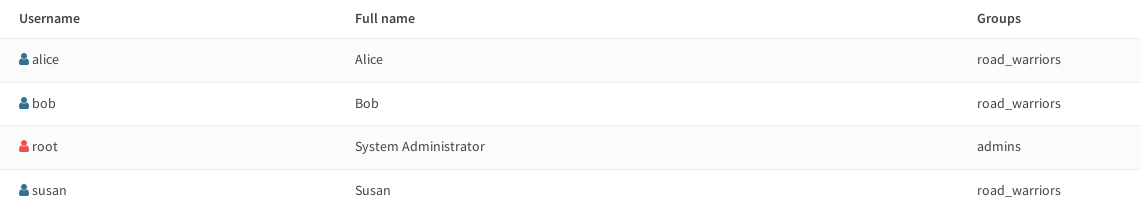
\includegraphics[width=\linewidth]{openvpn/users}
        \label{fig:users}
    \end{figure}
    \vspace{-20pt}
    Create the three new users \textit{alice}, \textit{bob} and \textit{susan} in System $\rightarrow$ Access $\rightarrow$ Users.
    All fields except username and password are optional and may be omitted. 
    Then, create the group \textit{road\_warriors} and add to it the newly created users.
    
    \subsection{Server}
    Create a new server in VPN $\rightarrow$ OpenVPN $\rightarrow$ Servers and populate it with the following options.
    The encryption settings provide additional security with respect to the default (except for the password-only authentication mode, which has been decided with smartphones in mind), while the subnet \texttt{10.10.0.0/24} has been chosen without a precise reason.
    \begin{figure}[H]
        \centering
        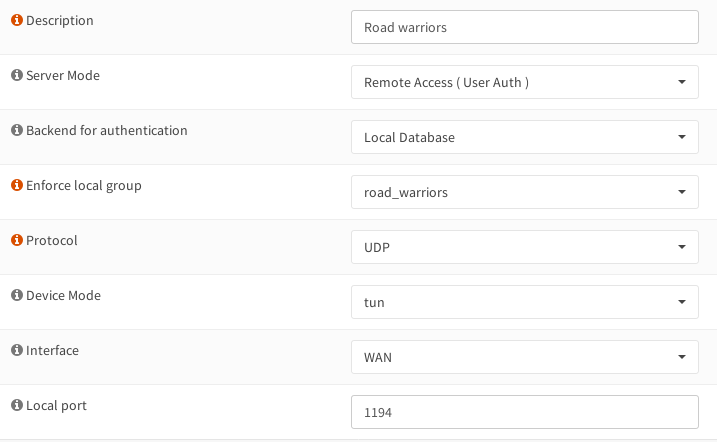
\includegraphics[width=\linewidth]{openvpn/settings-general}
        \label{fig:openvpn-settings-general}
    \end{figure}
    \vspace{-20pt}
    \begin{figure}[H]
        \centering
        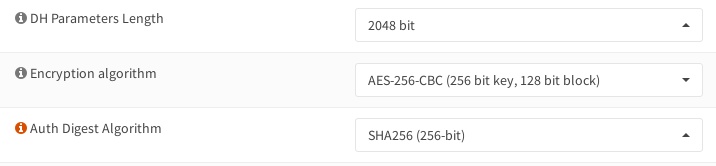
\includegraphics[width=\linewidth]{openvpn/settings-security}
        \label{fig:openvpn-settings-security}
    \end{figure}
    \vspace{-20pt}
    \begin{figure}[H]
        \centering
        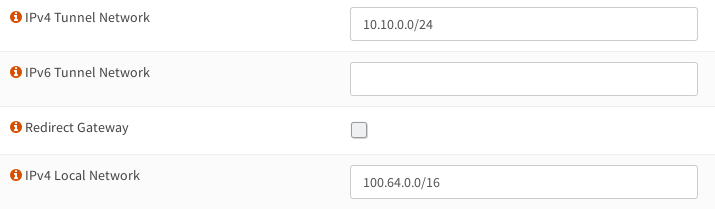
\includegraphics[width=\linewidth]{openvpn/settings-tunnel}
        \label{fig:openvpn-settings-tunnel}
    \end{figure}
    \vspace{-20pt}
    
    \subsection{Firewall rules}
    Firstly, it is necessary to allow incoming OpenVPN packets from the internet.
    To do so, create a new rule for interface WAN that accepts UDP packets with destination port 1194, the standard OpenVPN port.
    \begin{figure}[H]
        \centering
        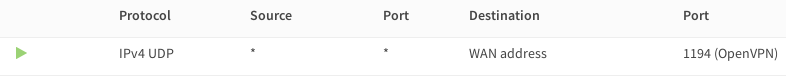
\includegraphics[width=\linewidth]{openvpn/rules-vpn}
        \label{fig:openvpn-rules-vpn}
    \end{figure}
    
    Then, allow access to \client and \ser networks for road warriors.
    Given that the specifics are not clear about the type of access the road warriors have and that they may have different needs than normal employees, allowing all TCP/UDP packets was considered a good compromise between security and functionality.
    
    In addition to creating the rules for the standard interfaces (those in \texttt{100.64.254.0/30}, \texttt{100.64.1.0/24} and \texttt{100.64.2.0/24}), we also define equivalent rules in the automatically-generated OpenVPN interface.
    \begin{figure}[H]
        \centering
        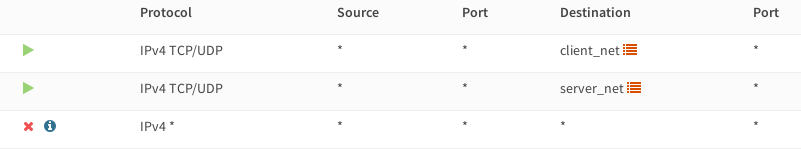
\includegraphics[width=\linewidth]{openvpn/rules-clients}
        \label{fig:rules-clients}
    \end{figure}
       
    \subsection{Clients}
    In VPN $\rightarrow$ OpenVPN $\rightarrow$ Client Export it is possible to download the OpenVPN configuration files.
    Obviously, it is necessary to insert the public IP for the WAN interface, which is usually fixed for enterprise networks.
    
    To start a new connection, execute the command \mintinline{sh}{openvpn --config FILE.ovpn} and insert a pair of valid credentials.
    \begin{figure}[H]
        \centering
        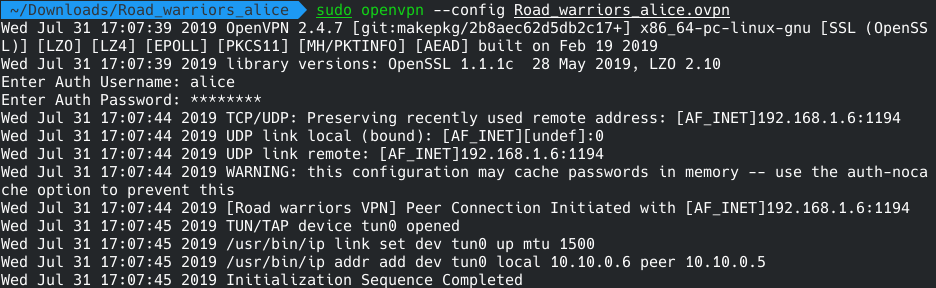
\includegraphics[width=\linewidth]{openvpn/client}
        \label{fig:openvpn-client}
    \end{figure}
    
    
    \section{VPN for the firewall tunnel}
    \subsection{Phase 1}
    In VPN $\rightarrow$ IPsec $\rightarrow$ Tunnel Settings create a new phase 1 connection.
    In the general settings, insert the following data for \mainfw and the inverse for \intfw.
    \begin{figure}[H]
        \centering
        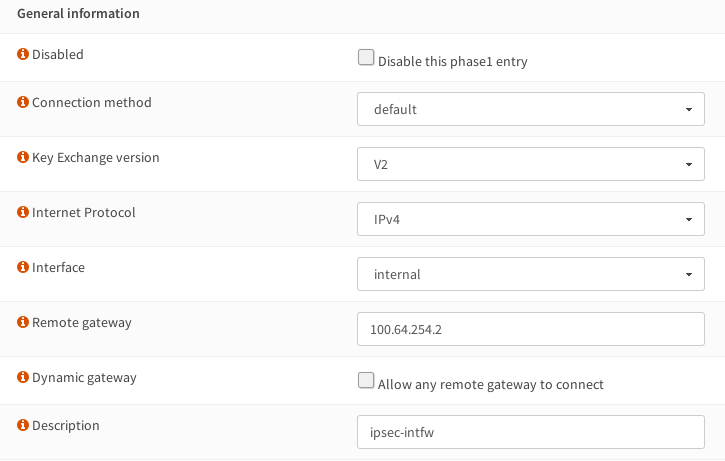
\includegraphics[width=\linewidth]{ipsec/phase1-general}
        \label{fig:ipsec-phase1-general}
    \end{figure}
    \vspace{-10pt}
%
    Proposal settings must be identical in both firewalls, otherwise the session negotiation will fail.
    \vspace{-5pt}
    \begin{figure}[H]
        \centering
        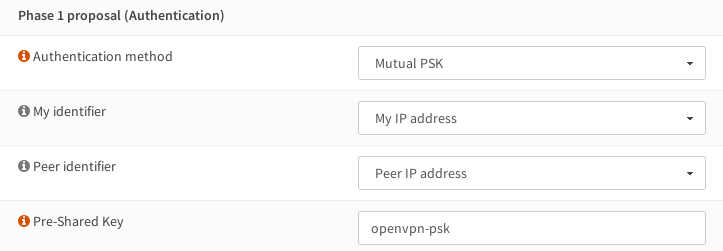
\includegraphics[width=\linewidth]{ipsec/phase1-proposal-auth}
        \label{fig:ipsec-phase1-proposal-auth}
    \end{figure}
    \begin{figure}[H]
        \centering
        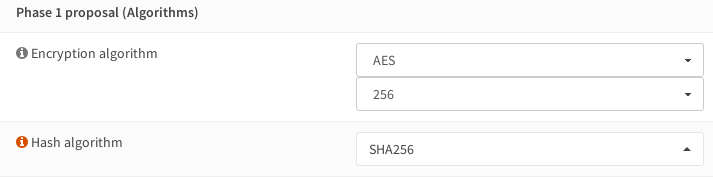
\includegraphics[width=\linewidth]{ipsec/phase1-proposal-alg}
        \label{fig:ipsec-phase1-proposal-alg}
    \end{figure}
    \vspace{-10pt}
%
    Since phase 2 will be route-based, untick the Install policy checkbox.
    \vspace{-5pt}
    \begin{figure}[H]
        \centering
        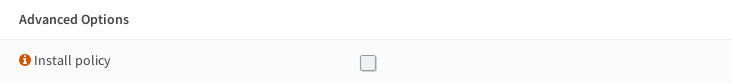
\includegraphics[width=\linewidth]{ipsec/phase1-advanced}
        \label{fig:ipsec-phase1-advanced}
    \end{figure}
    
    \subsection{Phase 2}
    In VPN $\rightarrow$ IPsec $\rightarrow$ Tunnel Settings, create a new phase 2 configuration.
    Since \intfw must use \mainfw as the default gateway, it is not possible to use a tunnel connection: the two networks must not overlap but \texttt{0.0.0.0/0} contains all possible subnets.
    Instead, use a route-based setup using the \texttt{100.64.254.0/30} addresses.
    \begin{figure}[H]
        \centering
        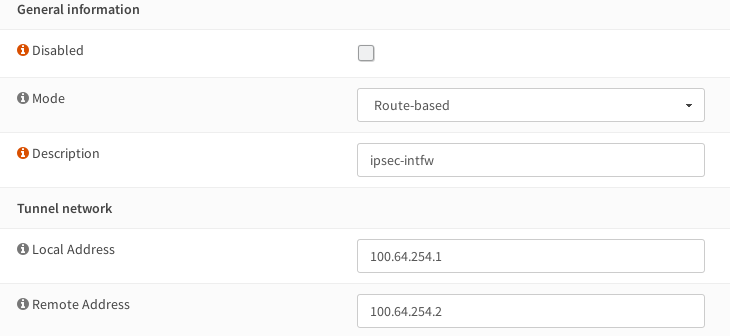
\includegraphics[width=\linewidth]{ipsec/phase2-general}
        \label{fig:ipsec-phase2-general}
    \end{figure}
%
    In both firewalls, in order to increase security set up the proposal settings as follows.
    MD5 and SHA1 are insecure and should be avoided, AES-128 is acceptable but AES-256 is better.
    \begin{figure}[H]
        \centering
        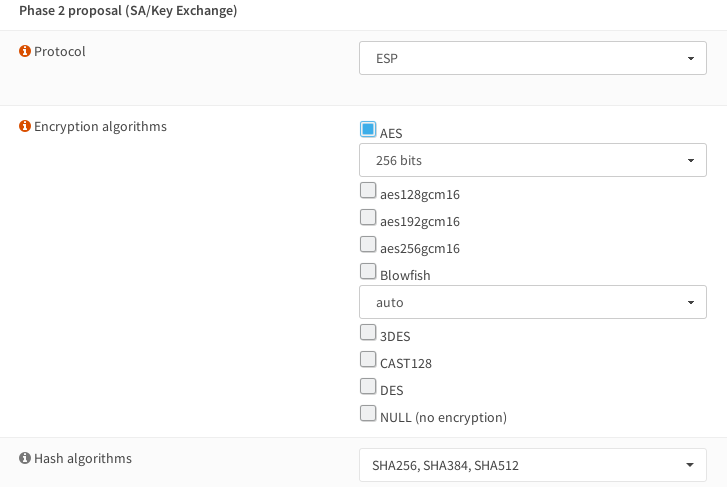
\includegraphics[width=\linewidth]{ipsec/phase2-proposal}
        \label{fig:ipsec-phase2-proposal}
    \end{figure}
    
    \subsection{Firewall rules}
    Transfer in both firewall the rules from the interfaces in \texttt{100.64.254.0/30} to the newly-generated IPsec ones.
    Add to the old interfaces the rules that allow IPsec traffic.
    \begin{figure}[H]
        \centering
        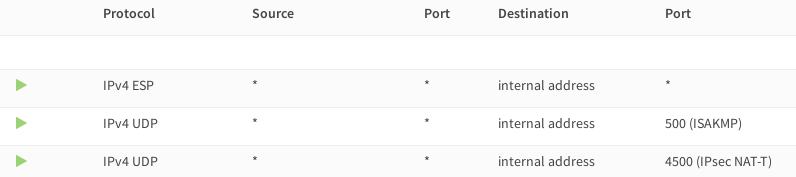
\includegraphics[width=\linewidth]{ipsec/rules}
        \label{fig:ipsec-rules}
    \end{figure}
    
    \subsection{Routes}
    In \mainfw, change the \texttt{100.64.0.0/16} route from the internal interface to the IPsec one.
    In \intfw, change the default gateway to the IPsec interface.
    
    
    \section{Test of the configuration}
    IPsec was tested with the same files as the previous laboratory because the allowed traffic did not change.
    For OpenVPN, a \texttt{road\_warriors.test} file, which uses the same return codes, was executed on the local machine.
    FTP and SSH services were tested manually for the reasons already expressed in the previous report.
    
    
    \section{Final remarks}
    OpenVPN is one of the most commonly used VPN protocols thanks to its security and ease of use.
    Therefore, it is a sensible choice for road warriors, since they must have a safe and reliable communication channel with the base office.
    
    IPsec, on the other hand, is less flexible and more difficult to configure.
    Since it encrypts IP packets, it is more suited to use cases where both endpoints are fixed.
    In this particular case, assuming that both firewalls are located in the same secure compound and that the communication channel does not leave its premises, IPsec is an overkill.
    The additional -- and superfluous -- security does not justify the substantial latency increase.
\end{document}
